    \section{Podobnost}

        
            \subsection*{Središčni razteg}

            \begin{definicija}
                \textbf{Središčni razteg} ali \textbf{homotetija} s središčem v neki točki $O$ in faktorjem $k\neq 0$ je podobnostna preslikava,
                ki daljico $OA$ preslika v daljico $OA'$, pri čemer velja $|OA'|=|k|\cdot|OA|$.

                \begin{figure}[H]
                    \centering
                    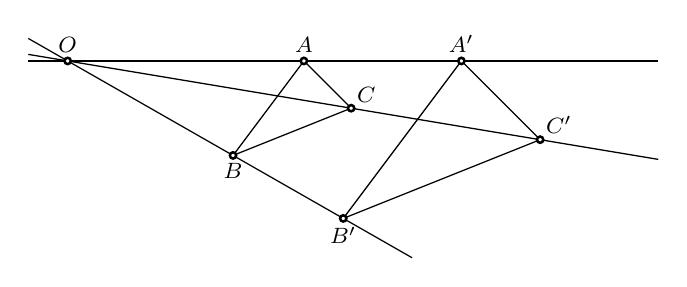
\begin{tikzpicture}
                    % \clip (0,0) rectangle (14.000000,10.000000);
                    {\footnotesize

                    % Drawing line O A
                    \draw [line width=0.016cm] (1.000000,3.500000) -- (1.460000,3.500000);%
                    \draw [line width=0.016cm] (1.540000,3.500000) -- (4.460000,3.500000);%
                    \draw [line width=0.016cm] (4.540000,3.500000) -- (6.460000,3.500000);%
                    \draw [line width=0.016cm] (6.540000,3.500000) -- (9.000000,3.500000);%

                    % Drawing line O B
                    \draw [line width=0.016cm] (5.875000,1.000000) -- (5.034730,1.480154);%
                    \draw [line width=0.016cm] (4.965270,1.519846) -- (3.634730,2.280154);%
                    \draw [line width=0.016cm] (3.565270,2.319846) -- (1.534730,3.480154);%
                    \draw [line width=0.016cm] (1.465270,3.519846) -- (1.000000,3.785714);%

                    % Drawing line O C
                    \draw [line width=0.016cm] (1.000000,3.583333) -- (1.460544,3.506576);%
                    \draw [line width=0.016cm] (1.539456,3.493424) -- (5.060544,2.906576);%
                    \draw [line width=0.016cm] (5.139456,2.893424) -- (7.460544,2.506576);%
                    \draw [line width=0.016cm] (7.539456,2.493424) -- (9.000000,2.250000);%

                    % Drawing segment A B
                    \draw [line width=0.016cm] (4.476000,3.468000) -- (3.624000,2.332000);%

                    % Drawing segment B C
                    \draw [line width=0.016cm] (3.637139,2.314856) -- (5.062861,2.885144);%

                    % Drawing segment A C
                    \draw [line width=0.016cm] (4.528284,3.471716) -- (5.071716,2.928284);%

                    % Drawing segment A' B'
                    \draw [line width=0.016cm] (6.476000,3.468000) -- (5.024000,1.532000);%

                    % Drawing segment B' C'
                    \draw [line width=0.016cm] (5.037139,1.514856) -- (7.462861,2.485144);%

                    % Drawing segment A' C'
                    \draw [line width=0.016cm] (6.528284,3.471716) -- (7.471716,2.528284);%

                    % Marking point O by circle
                    \draw [line width=0.032cm] (1.500000,3.500000) circle (0.040000);%
                    \draw (1.500000,3.500000) node [anchor=south] { $O$ };%

                    % Marking point A by circle
                    \draw [line width=0.032cm] (4.500000,3.500000) circle (0.040000);%
                    \draw (4.500000,3.500000) node [anchor=south] { $A$ };%

                    % Marking point A' by circle
                    \draw [line width=0.032cm] (6.500000,3.500000) circle (0.040000);%
                    \draw (6.500000,3.500000) node [anchor=south] { $A'$ };%

                    % Marking point B by circle
                    \draw [line width=0.032cm] (3.600000,2.300000) circle (0.040000);%
                    \draw (3.600000,2.300000) node [anchor=north] { $B$ };%

                    % Marking point B' by circle
                    \draw [line width=0.032cm] (5.000000,1.500000) circle (0.040000);%
                    \draw (5.000000,1.500000) node [anchor=north] { $B'$ };%

                    % Marking point C by circle
                    \draw [line width=0.032cm] (5.100000,2.900000) circle (0.040000);%
                    \draw (5.070000,2.870000) node [anchor=south west] { $C$ };%

                    % Marking point C' by circle
                    \draw [line width=0.032cm] (7.500000,2.500000) circle (0.040000);%
                    \draw (7.470000,2.470000) node [anchor=south west] { $C'$ };%
                    }
                    \end{tikzpicture}
                \end{figure}


                $$ |OA'|:|OA|=k \quad\quad |OB'|:|OB|=k \quad\quad |OC'|:|OC|=k $$
                $$ |A'B'|:|AB|=k \quad\quad |B'C'|:|BC|=k \quad\quad |A'C'|:|AC|=k $$
            \end{definicija}
            

        
        
            \subsubsection*{Lastnosti}
                Središčni razteg s središčem v točki $O$ in faktorjem $k\neq 0$:
                \begin{itemize}
                    \item ohranja velikosti kotov;
                    \item vse razdalje pomnoži s $|k|$, pri čemer:
                        \begin{itemize}
                            \item $|k|>1$ pomeni razteg,
                            \item $k=1$ pomeni identiteto,
                            \item $|k|<1$ pomeni skrčitev,
                            \item $k=-1$ pomeni zrcaljenje čez točko $O$;
                        \end{itemize}
                    \item premico preslika v vzporedno premico;
                    \item daljico $AB$ preslika na vzporedno daljico $A'B'$;
                    \item ohranja premice, ki gredo skozi točko $O$.
                \end{itemize}
            
        


        
            \subsection*{Podobnost}


            \begin{definicija}
                \textbf{Podobnostna preslikava} je preslikava, sestavljena iz togega premika in središčnega raztega.
            \end{definicija}

            \begin{definicija}
                Dva lika sta \textbf{podobna}, če med njima obstaja podobnostna preslikava.
            \end{definicija}

            
            Podobnost je v množici ravninskih likov \textit{ekvivalenčna relacija}, saj je:
                \begin{itemize}
                    \item \textit{refleksivna}: $L\sim L$ -- vsaka množica je podobna sami sebi (koeficient podobnosti $k=1$);
                    \item \textit{simetrična}: $L\sim L' \Rightarrow L'\sim L$ -- če je prva množica podobna drugi, je tudi druga podobna prvi (koeficienta podobnosti $k$ in $\frac{1}{k}$);
                    \item \textit{tranzitivna}: $L\sim L' \land L'\sim L'' \rightarrow L\sim L''$ -- če je prva množica podobna drugi in druga podobna tretji, 
                            je tudi prva množica podobna tretji množici (koeficienti podobnosti $k_1$, $k_2$ in $k_1k_2$).
                \end{itemize}
            

        


        
            \begin{izrek}[Talesov izrek o sorazmerjih]
                Če premici, ki se sekata v eni točki, sekamo z množico vzporednic, 
                je razmerje odsekov na eni premici šopa enako razmerju enakoležnih odsekov na drugi premici istega šopa.

                \begin{figure}[H]
                    \centering
                    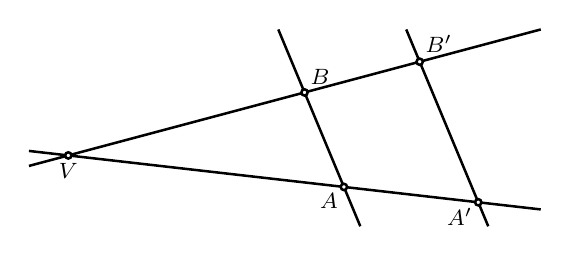
\begin{tikzpicture}
                    % \clip (0,0) rectangle (14.000000,10.000000);
                    {\footnotesize

                    % Marking point V by circle
                    \draw [line width=0.032cm] (1.500000,1.900000) circle (0.040000);%
                    \draw (1.500000,1.900000) node [anchor=north] { $V$ };%

                    % Marking point A by circle
                    \draw [line width=0.032cm] (5.000000,1.500000) circle (0.040000);%
                    \draw (5.030000,1.530000) node [anchor=north east] { $A$ };%

                    % Marking point B by circle
                    \draw [line width=0.032cm] (4.500000,2.700000) circle (0.040000);%
                    \draw (4.470000,2.700000) node [anchor=south west] { $B$ };%

                    % Drawing line a
                    \draw [line width=0.032cm] (1.000000,1.957143) -- (1.460259,1.904542);%
                    \draw [line width=0.032cm] (1.539741,1.895458) -- (4.960259,1.504542);%
                    \draw [line width=0.032cm] (5.039741,1.495458) -- (6.666509,1.309542);%
                    \draw [line width=0.032cm] (6.745991,1.300458) -- (7.500000,1.214286);%

                    % Drawing line b
                    \draw [line width=0.032cm] (7.500000,3.500000) -- (6.001149,3.100307);%
                    \draw [line width=0.032cm] (5.923851,3.079693) -- (4.538649,2.710307);%
                    \draw [line width=0.032cm] (4.461351,2.689693) -- (1.538649,1.910307);%
                    \draw [line width=0.032cm] (1.461351,1.889693) -- (1.000000,1.766667);%

                    % Marking point A' by circle
                    \draw [line width=0.032cm] (6.706250,1.305000) circle (0.040000);%
                    \draw (6.736250,1.335000) node [anchor=north east] { $A'$ };%

                    % Marking point B' by circle
                    \draw [line width=0.032cm] (5.962500,3.090000) circle (0.040000);%
                    \draw (5.932500,3.100000) node [anchor=south west] { $B'$ };%

                    % Drawing line A B
                    \draw [line width=0.032cm] (5.208333,1.000000) -- (5.015385,1.463077);%
                    \draw [line width=0.032cm] (4.984615,1.536923) -- (4.515385,2.663077);%
                    \draw [line width=0.032cm] (4.484615,2.736923) -- (4.166667,3.500000);%

                    % Drawing line A' B'
                    \draw [line width=0.032cm] (6.833333,1.000000) -- (6.721635,1.268077);%
                    \draw [line width=0.032cm] (6.690865,1.341923) -- (5.977885,3.053077);%
                    \draw [line width=0.032cm] (5.947115,3.126923) -- (5.791667,3.500000);%
                    }
                    \end{tikzpicture}
                \end{figure}


                $$ |VA|:|VA'|=|VB|:|VB'| $$
                $$ |VA|:|AB|=|VA'|:|A'B'| $$
                $$ |VA|:|AA'|=|VB|:|BB'| $$
            \end{izrek}
        


        
            \subsection*{Podobnost trikotnikov}


            \begin{definicija}
                Trikotnika $\triangle ABC$ in $\triangle A'B'C'$ sta podobna, če imata enaka razmerja vseh istoležnih stranic in enake vse notranje kote.

                \begin{figure}[H]
                    \centering
                    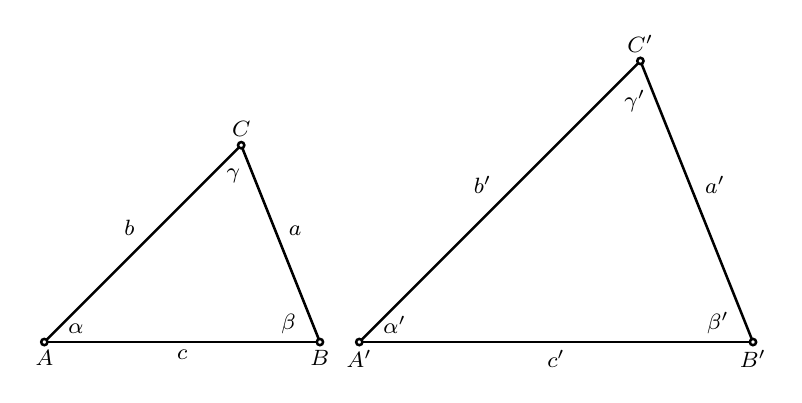
\begin{tikzpicture}
                    % \clip (0,0) rectangle (14.000000,10.000000);
                    {\footnotesize

                    % Marking point \alpha
                    \draw (1.700000,1.500000) node [anchor=south west] { $\alpha$ };%

                    % Marking point \alpha'
                    \draw (5.700000,1.500000) node [anchor=south west] { $\alpha'$ };%

                    % Marking point \beta
                    \draw (4.800000,1.500000) node [anchor=south east] { $\beta$ };%

                    % Marking point \beta'
                    \draw (10.300000,1.500000) node [anchor=south east] { $\beta'$ };%

                    % Marking point \gamma
                    \draw (3.900000,3.800000) node [anchor=north] { $\gamma$ };%

                    % Marking point \gamma'
                    \draw (9.000000,4.800000) node [anchor=north] { $\gamma'$ };%

                    % Marking point c
                    \draw (3.250000,1.500000) node [anchor=north] { $c$ };%

                    % Marking point c'
                    \draw (8.000000,1.500000) node [anchor=north] { $c'$ };%

                    % Marking point a
                    \draw (4.500000,2.750000) node [anchor=south west] { $a$ };%

                    % Marking point a'
                    \draw (9.785000,3.285000) node [anchor=south west] { $a'$ };%

                    % Marking point b
                    \draw (2.750000,2.750000) node [anchor=south east] { $b$ };%

                    % Marking point b'
                    \draw (7.285000,3.285000) node [anchor=south east] { $b'$ };%

                    % Drawing segment A B
                    \draw [line width=0.032cm] (1.540000,1.500000) -- (4.960000,1.500000);%

                    % Drawing segment B C
                    \draw [line width=0.032cm] (4.985144,1.537139) -- (4.014856,3.962861);%

                    % Drawing segment A C
                    \draw [line width=0.032cm] (1.528284,1.528284) -- (3.971716,3.971716);%

                    % Marking point A by circle
                    \draw [line width=0.032cm] (1.500000,1.500000) circle (0.040000);%
                    \draw (1.500000,1.500000) node [anchor=north] { $A$ };%

                    % Marking point B by circle
                    \draw [line width=0.032cm] (5.000000,1.500000) circle (0.040000);%
                    \draw (5.000000,1.500000) node [anchor=north] { $B$ };%

                    % Marking point C by circle
                    \draw [line width=0.032cm] (4.000000,4.000000) circle (0.040000);%
                    \draw (4.000000,4.000000) node [anchor=south] { $C$ };%

                    % Drawing segment A' B'
                    \draw [line width=0.032cm] (5.540000,1.500000) -- (10.460000,1.500000);%

                    % Drawing segment B' C'
                    \draw [line width=0.032cm] (10.485126,1.537132) -- (9.084874,5.032868);%

                    % Drawing segment A' C'
                    \draw [line width=0.032cm] (5.528284,1.528284) -- (9.041716,5.041716);%

                    % Marking point A' by circle
                    \draw [line width=0.032cm] (5.500000,1.500000) circle (0.040000);%
                    \draw (5.500000,1.500000) node [anchor=north] { $A'$ };%

                    % Marking point B' by circle
                    \draw [line width=0.032cm] (10.500000,1.500000) circle (0.040000);%
                    \draw (10.500000,1.500000) node [anchor=north] { $B'$ };%

                    % Marking point C' by circle
                    \draw [line width=0.032cm] (9.070000,5.070000) circle (0.040000);%
                    \draw (9.070000,5.070000) node [anchor=south] { $C'$ };%
                    }
                    \end{tikzpicture}
                \end{figure}


                $$ a:b:c=a':b':c' \quad \land \quad \alpha=\alpha', \beta=\beta', \gamma=\gamma' \quad \Rightarrow \quad \triangle ABC \sim \triangle A'B'C' $$
            \end{definicija}


        

        
        
            \begin{izrek}[o podobnosti trikotnikov]
                Dva trikotnika sta si podobna, če se ujemata:
                \begin{enumerate}
                    \item v razmerjih po dveh enakoležnih stranic ($a:a'=b:b'=c:c'=k$);
                    \item v dveh notranjih kotih (npr. $\alpha=\alpha'$, $\beta=\beta'$);
                    \item v razmerju dveh stranic in v vmesnem kotu (npr. $b:c=b':c'$, $\alpha=\alpha'$);
                    \item v razmerju dveh stranic in v kotu nasproti daljše.
                \end{enumerate}
            \end{izrek}

            \begin{izrek}
                Podobna trikotnika imata sorazmerna obsega, koeficient podobnosti je $k$, isti kot za dolžine stranic.
                Sorazmerni sta tudi višini trikotnikov.

                Ploščini podobnih trikotnikov sta sorazmerni s koeficientom podobnosti $k^2$.
            \end{izrek}
        

        
        
            \subsection*{Izreki v pravokotnem trikotniku}


            
                \begin{figure}[H]
                    \centering
                    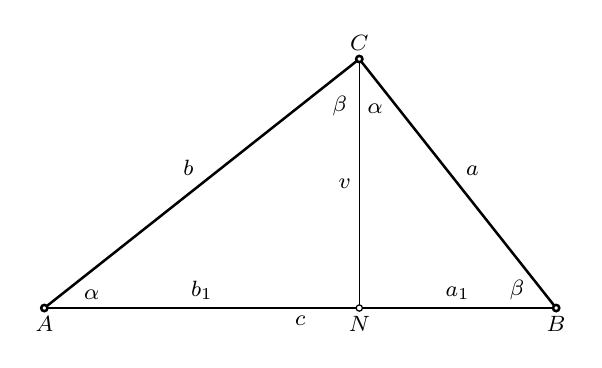
\begin{tikzpicture}
                    % \clip (0,0) rectangle (14.000000,10.000000);
                    {\footnotesize

                    % Marking point v
                    \draw (5.500000,3.081139) node [anchor=east] { $v$ };%

                    % Marking point b
                    \draw (3.500000,3.081139) node [anchor=south east] { $b$ };%

                    % Marking point a
                    \draw (6.750000,3.081139) node [anchor=south west] { $a$ };%

                    % Marking point c
                    \draw (4.750000,1.500000) node [anchor=north] { $c$ };%

                    % Marking point a_1
                    \draw (3.500000,1.500000) node [anchor=south] { $b_1$ };%

                    % Marking point b_1
                    \draw (6.750000,1.500000) node [anchor=south] { $a_1$ };%

                    % Marking point \alpha
                    \draw (1.900000,1.500000) node [anchor=south west] { $\alpha$ };%

                    % Marking point \beta
                    \draw (7.700000,1.500000) node [anchor=south east] { $\beta$ };%

                    % Marking point \alpha
                    \draw (5.500000,4.200000) node [anchor=north west] { $\alpha$ };%

                    % Marking point \beta
                    \draw (5.450000,4.300000) node [anchor=north east] { $\beta$ };%

                    % Drawing segment C N
                    \draw [line width=0.016cm] (5.500000,4.622278) -- (5.500000,1.540000);%

                    % Marking point N by circle
                    \draw [line width=0.016cm] (5.500000,1.500000) circle (0.040000);%
                    \draw (5.500000,1.500000) node [anchor=north] { $N$ };%

                    % Drawing segment A B
                    \draw [line width=0.032cm] (1.540000,1.500000) -- (5.460000,1.500000);%
                    \draw [line width=0.032cm] (5.540000,1.500000) -- (7.960000,1.500000);%

                    % Drawing segment A C
                    \draw [line width=0.032cm] (1.531379,1.524807) -- (5.468621,4.637471);%

                    % Drawing segment B C
                    \draw [line width=0.032cm] (7.975193,1.531379) -- (5.524807,4.630899);%

                    % Marking point A by circle
                    \draw [line width=0.032cm] (1.500000,1.500000) circle (0.040000);%
                    \draw (1.500000,1.500000) node [anchor=north] { $A$ };%

                    % Marking point B by circle
                    \draw [line width=0.032cm] (8.000000,1.500000) circle (0.040000);%
                    \draw (8.000000,1.500000) node [anchor=north] { $B$ };%

                    % Marking point C by circle
                    \draw [line width=0.032cm] (5.500000,4.662278) circle (0.040000);%
                    \draw (5.500000,4.662278) node [anchor=south] { $C$ };%
                    }
                    \end{tikzpicture}
                \end{figure}
            

            \begin{izrek}[višinski izrek]
                Kvadrat višine v pravokotnem trikotniku je enak produktu pravokotnih projekcij katet na hipotenuzo.
                $$ v^2=a_1b_1 $$
            \end{izrek}        

            \begin{izrek}[Evklidov izrek]
                Kvadrat katete v pravokotnem trikotniku je enak produktu hipotenuze in pravokotne projekcije te katete na hipotenuzo.
                $$ a^2=a_1c \quad \text{in} \quad b^2=b_1c $$
            \end{izrek}

            \begin{izrek}[Pitagorov izrek]
                Kvadrat hipotenuze v pravokotnem trikotniku je enak vsoti kvadratov obeh katet.
                $$ c^2=a^2+b^2 $$
            \end{izrek}

        

        

        
